\chapter{绪论}\label{chap:introduction}

\section{研究背景与意义}

在全球科技迅猛发展的浪潮中，机器人技术（Robotics）已崛起为驱动社会进步与产业变革的核心驱动力。习近平总书记深刻指出，要“以科技创新推动产业创新，积极培育新能源、新材料、先进制造、电子信息等战略性新兴产业，积极培育未来产业，加快形成新质生产力，增强发展新动能”。作为衡量国家科技创新与高端制造水平的关键标志，机器人技术不仅是军事与商业领域的前沿焦点，更是全球竞逐的战略新高地。对此，我国政府高度重视，连续出台多项政策，旨在系统推进机器人技术的自主创新与深度应用。《“十四五”机器人产业发展规划》\cite{miit2021} 强调了机器人技术在制造业、服务行业和特种领域的应用，并提出了到 2025 年实现制造业机器人密度较 2020 年翻番的目标。工信部 2023 年发布的《“机器人+”应用行动实施方案》\cite{miit2023} 进一步提出，到 2025 年制造业机器人密度较 2020 年实现翻番。

地面移动机器人作为现有机器人中的绝对主流，越来越多地被用于工业生产、生活娱乐、搜救任务、军事侦察等场景中。在地面移动机器人的众多构型中，轮式机器人具有运动速度快、控制简单、能耗低等优点，但在非结构化地形（如楼梯、碎石、斜坡等）中的适应能力较差；而足式机器人虽具备良好的越障能力，但在平坦环境中运行时，在能效和运动速度方面落后于轮式机器人。为兼顾轮式机器人的高效性与足式机器人的地形适应性，轮足复合式机器人成为当前机器人研究的热点之一\cite{ding2024}。当前，主流研究聚焦于四足轮腿式机器人\cite{hutter2016}。该类机器人采用分布式腿部关节与轮组相耦合的设计，兼具动态平衡能力与中等障碍物跨越性能。然而，其多足架构也引发了结构冗余问题。以典型四足轮腿式机器人为例，其通常需配置 16 个以上的独立执行器，这不仅导致机械结构复杂性呈指数增长，还引入了显著的转动惯量与惯性负载，在控制器设计与建模上也带来了困难。而双轮足机器人作为一种典型的轮足融合构型，既能在平坦路面实现快速移动，又能通过腿部结构实现越障、上下楼梯等复杂动作，在结构上更加简单，具有重要的研究价值与应用前景。

在双轮足机器人机械结构上，主流设计分为串联、并联和混合式。串联结构工作空间大，但刚度和承载能力偏弱；并联结构刚度和承载力强，但运动空间受限。因此，本研究选择了混合式结构作为方向，它通过在串联主链中引入局部并联支链，旨在兼顾运动灵活性与结构刚性，从硬件基础上优化机器人的性能。在运动控制上，像 WBC（全身控制）、MPC（模型预测控制）这类高级算法虽然性能强大，但它们严重依赖高精度模型，计算复杂；而强化学习（RL）则需要海量的训练数据。这些都对机器人的实时控制和嵌入式部署提出了挑战。因此，本文将研究一种轻量级混合控制方案，以期在保证性能的同时，实现更高效的实时控制。总体来说，本课题旨在完成双轮足机器人的混合式腿部结构设计，同时提出一种面向嵌入式实时实现的分层轻量级混合控制方案：以 LQR（线性二次调节器）实现平衡、速度跟踪和腿摆控制量分配，以 VMC（虚拟模型控制）实现腿长方向支撑，结合基于滚转角几何关系的腿长差补偿提升侧向稳定性。

\section{双轮足机器人研究现状}

\subsection{机械结构}

\subsubsection{串联结构}

串联构型以开链关节实现大范围运动，控制灵活，是双轮足机器人最常见的腿部形式。波士顿动力 2017 年推出的 Handle\cite{boston2023handle}（\figref{fig:handle}）是串联轮腿机构的标杆，通过髋-膝-踝串联关节实现轮式平衡与跳跃越障，但其腿部惯量大，依赖高功率密度驱动。浙江大学 2023 年公开的 HotWheel\cite{yu2023hotwheel}（\figref{fig:hotwheel-serial}）在串联腿中增加了侧摆自由度（共 3 个主动自由度），扩展了足端工作空间，能在 V 型斜坡上稳定驻留。逐际动力 2024 年推出的 TRON 1\cite{limx2025tron1}（\figref{fig:tron1}）采用三自由度串联腿配合可更换足端，实现了点足、双足和双轮足的多形态切换。

\begin{figure}[H]
  \centering
  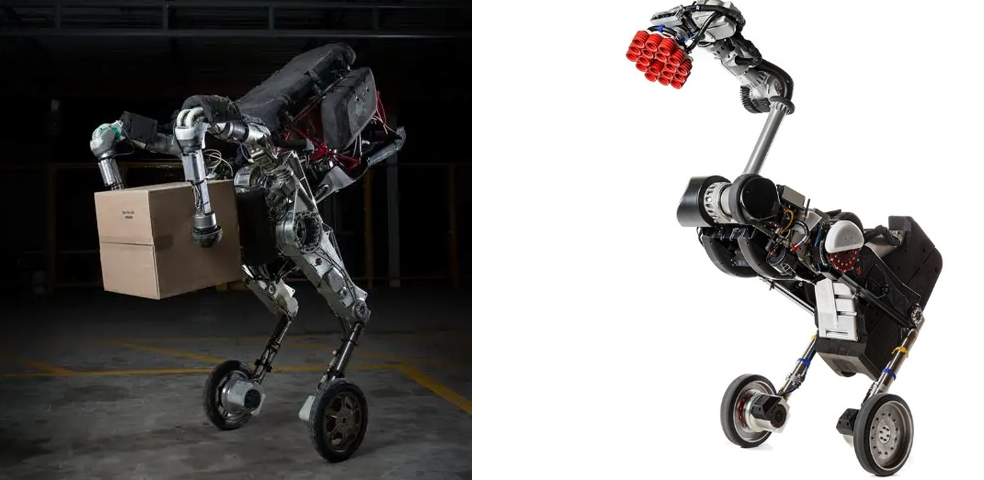
\includegraphics[width=0.7\textwidth]{figures/ch01/image3.png}
  \caption{一代 Handle 机器人（左），二代 Handle 机器人（右）\cite{boston2023handle,boston2023stretch}}
  \label{fig:handle}
\end{figure}

\begin{figure}[H]
  \centering
  \begin{minipage}[b]{0.4\textwidth}
    \centering
    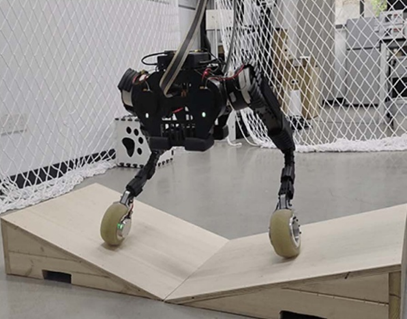
\includegraphics[width=\textwidth]{figures/ch01/image4.png}
  \end{minipage}
  \begin{minipage}[b]{0.4\textwidth}
    \centering
    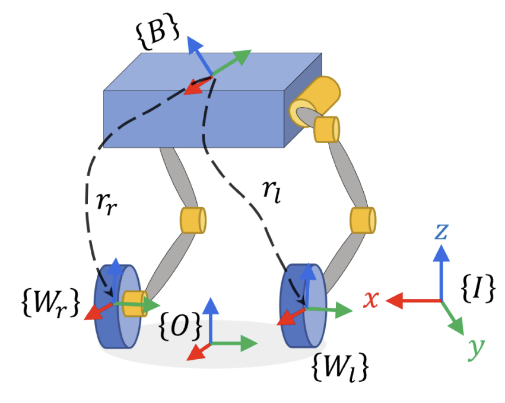
\includegraphics[width=\textwidth]{figures/ch01/image5.png}
  \end{minipage}
  \caption{HotWheel 机器人\cite{yu2023hotwheel}}
  \label{fig:hotwheel-serial}
\end{figure}

\begin{figure}[H]
  \centering
  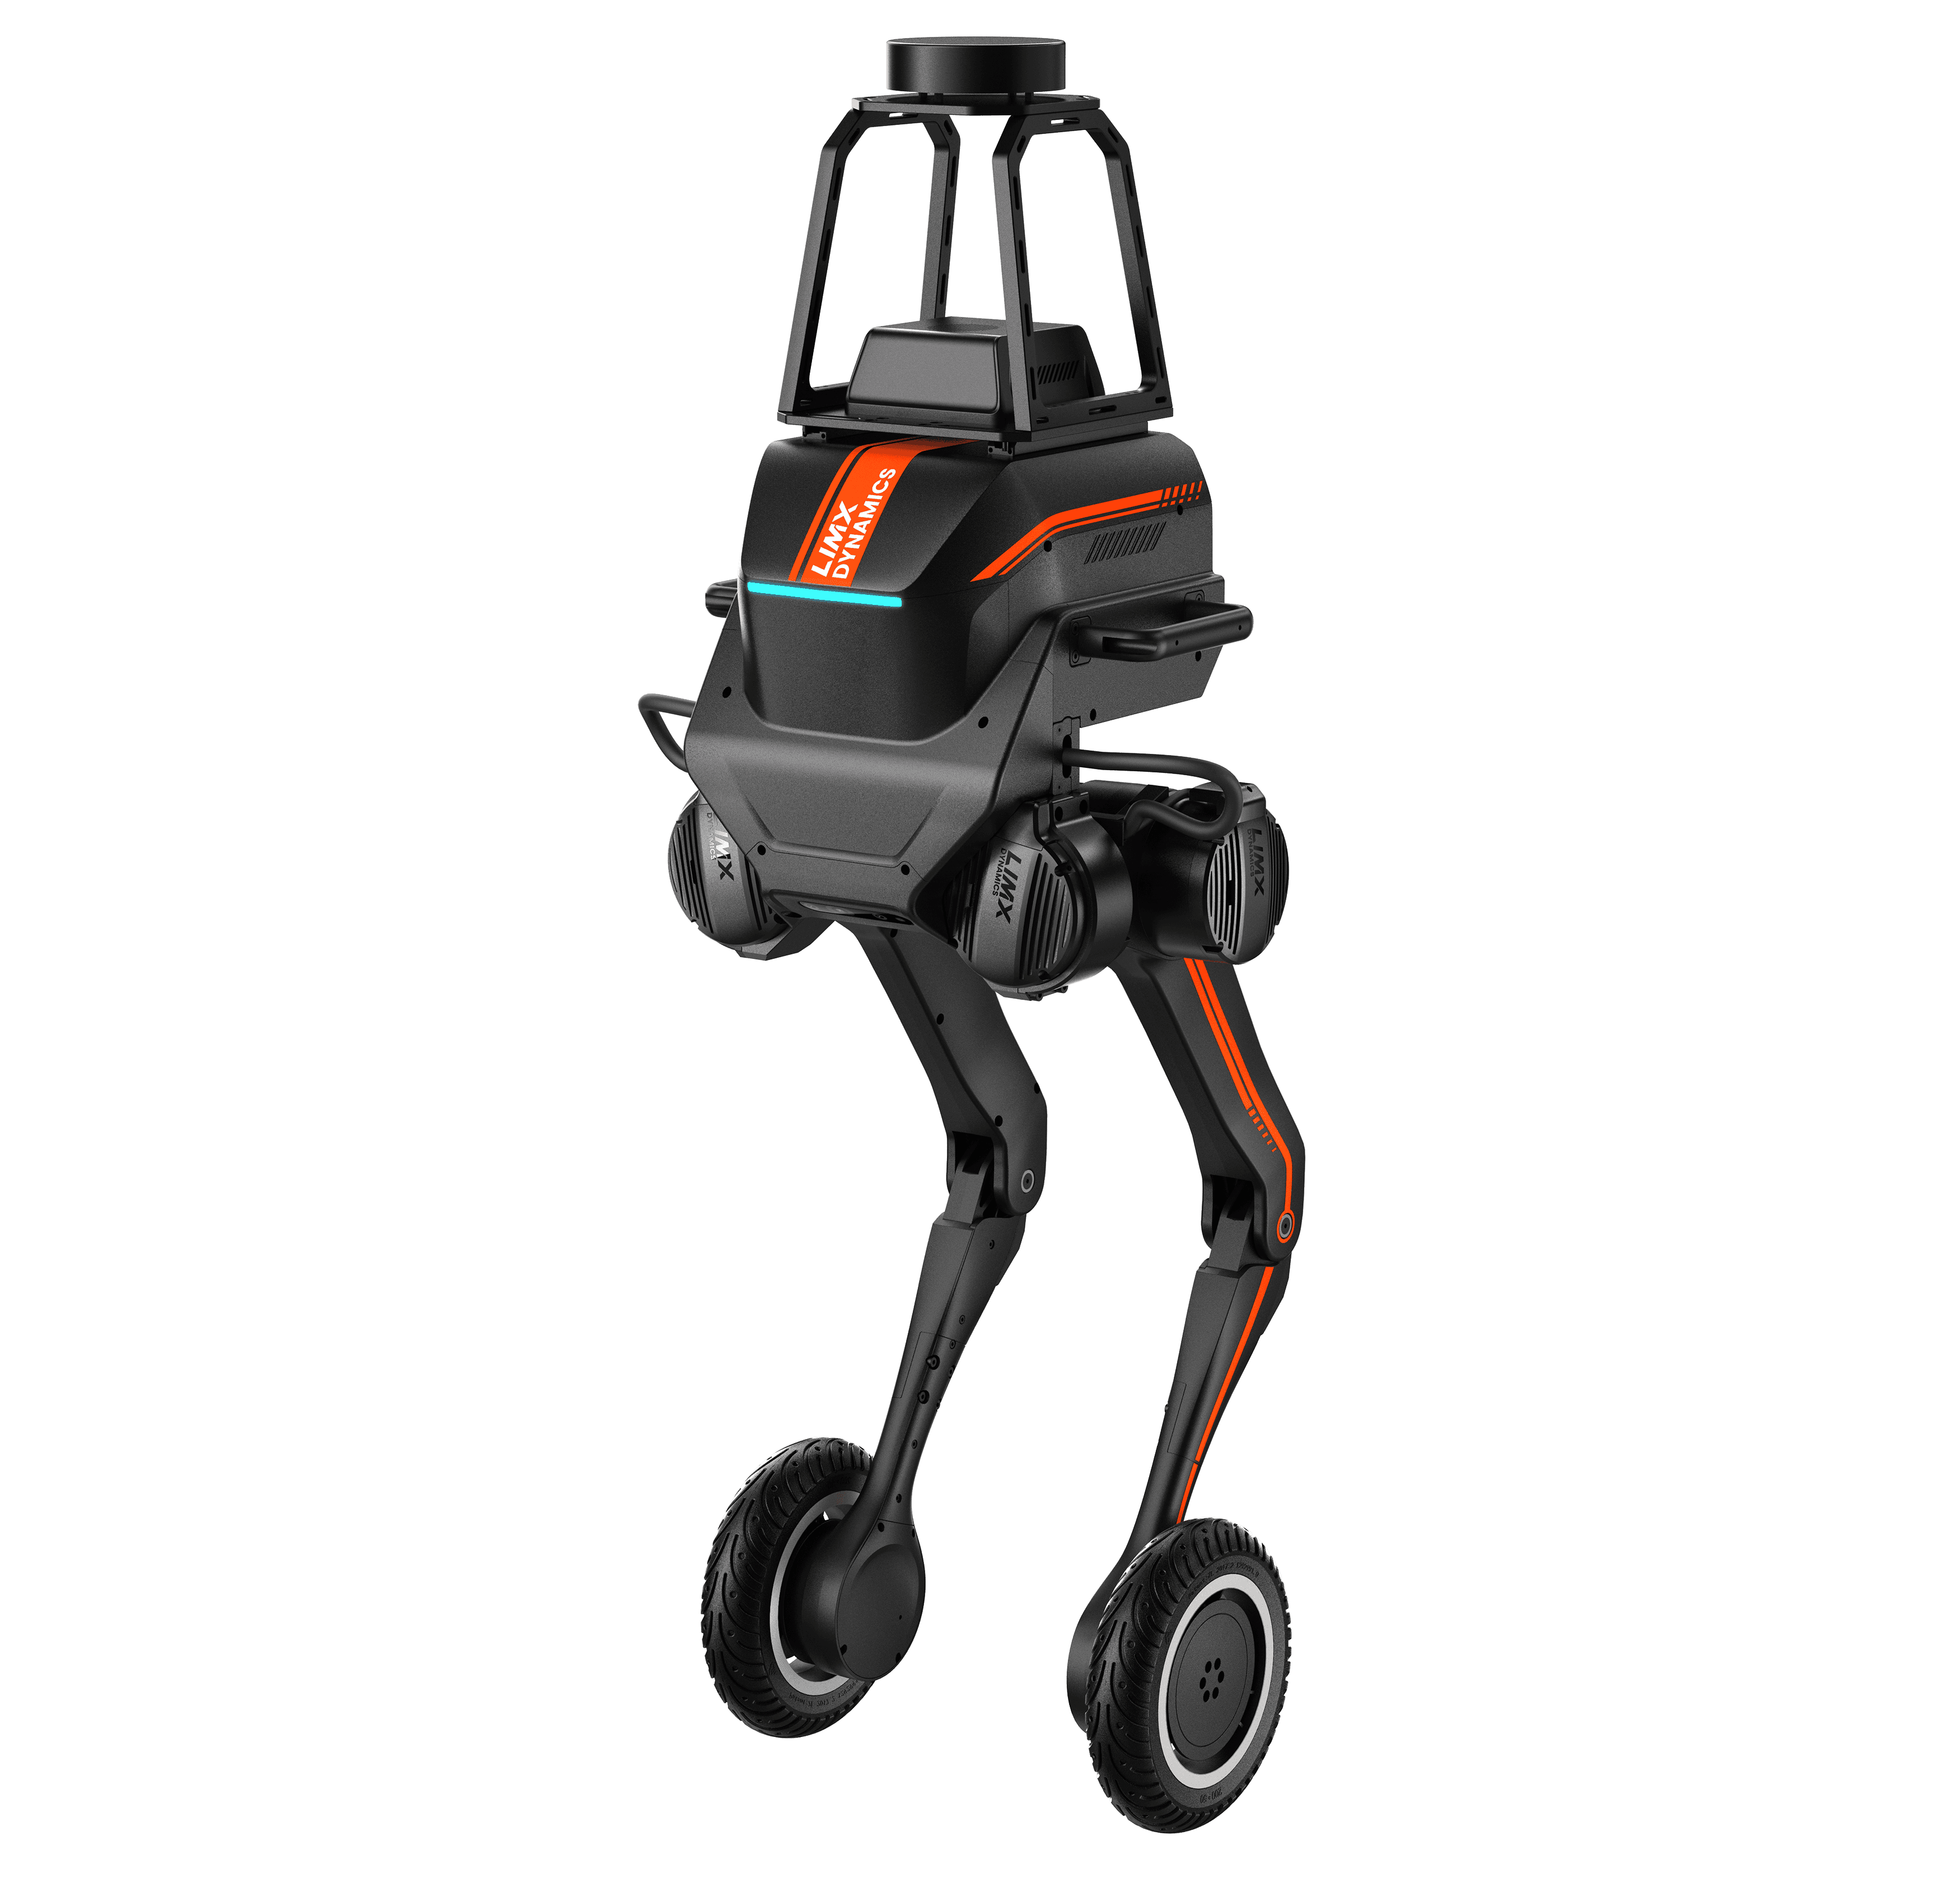
\includegraphics[width=0.5\textwidth]{figures/ch01/image6.png}
  \caption{TRON 1 机器人\cite{limx2025tron1}}
  \label{fig:tron1}
\end{figure}

上述平台的共性问题在于：开链结构导致腿部转动惯量偏高，串联关节逐级累积误差降低了整机刚度与末端定位精度。本文在机械设计中同样采用了串联主链以保留工作空间优势，但通过引入局部闭环支链来分担关节负载和提升侧向刚度，正是针对上述不足的改进尝试。

\subsubsection{并联结构}

并联构型以闭链机构提供高刚度和强承载能力，但工作空间受限。Sugahara 与 Hashimoto 团队在 2004--2005 年开发的 WL-16 与 WS-2 组合系统\cite{sugahara2004,hashimoto2005}（\figref{fig:ws2-wl16}）采用 6 自由度并联腿，通过切换足底橡胶垫的收放实现步态与轮式移动的切换，是早期轮足复合的代表。ETH Zurich 2019 年推出的 Ascento\cite{klemm2019ascento}（\figref{fig:ascento}）采用闭式四连杆机构，轮心近似直线运动，有效解耦了跳跃与平衡控制，并通过拓扑优化实现轻量化。腾讯 2021 年发布的 Ollie\cite{wang2021ollie}（\figref{fig:ollie}）采用对称五连杆设计，单腿集成一个轮毂电机与两个关节电机，腹部飞轮用于补偿空中姿态，能以 0.35\,m 最低身高完成空翻和跳跃。

\begin{figure}[H]
  \centering
  \begin{minipage}[b]{0.22\textwidth}
    \centering
    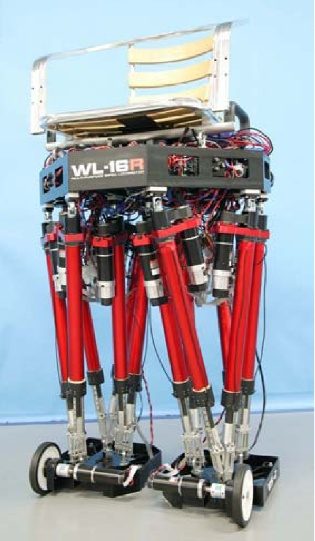
\includegraphics[width=\textwidth]{figures/ch01/image7.jpeg}
  \end{minipage}
  \begin{minipage}[b]{0.45\textwidth}
    \centering
    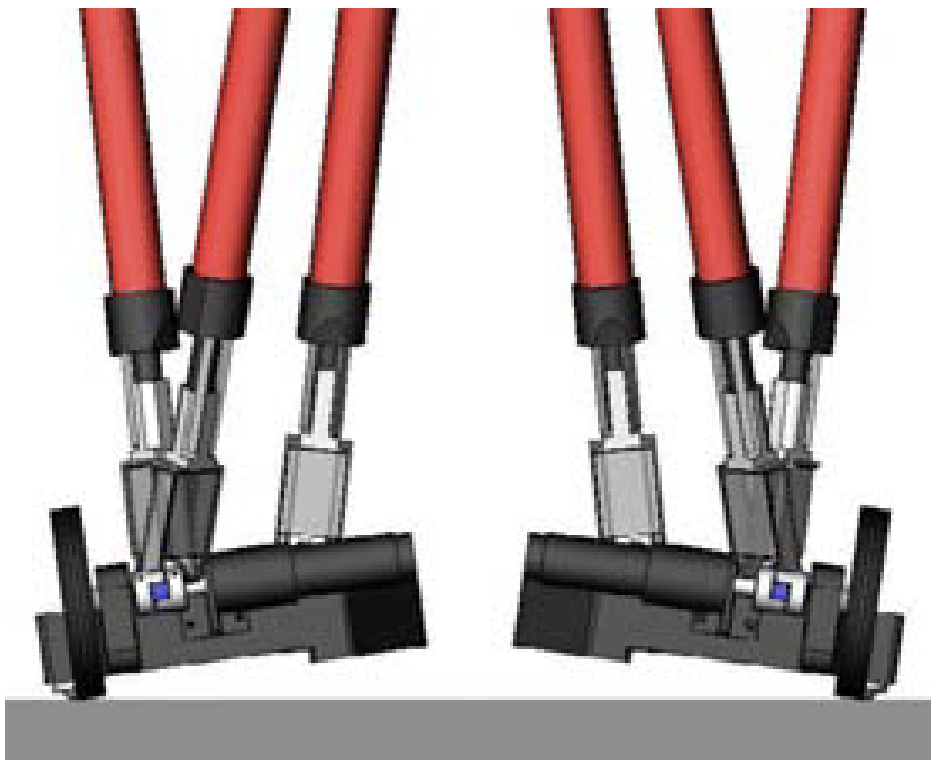
\includegraphics[width=\textwidth]{figures/ch01/image8.png}
  \end{minipage}
  \caption{WS-2 / WL-16\cite{sugahara2004,hashimoto2005}}
  \label{fig:ws2-wl16}
\end{figure}

\begin{figure}[H]
  \centering
  \begin{minipage}[b]{0.35\textwidth}
    \centering
    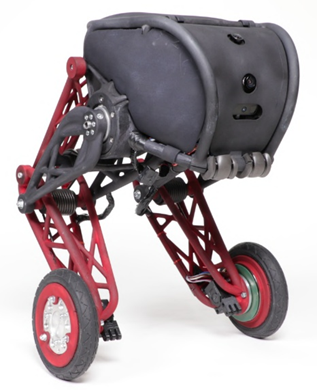
\includegraphics[width=\textwidth]{figures/ch01/image9.png}
  \end{minipage}
  \begin{minipage}[b]{0.5\textwidth}
    \centering
    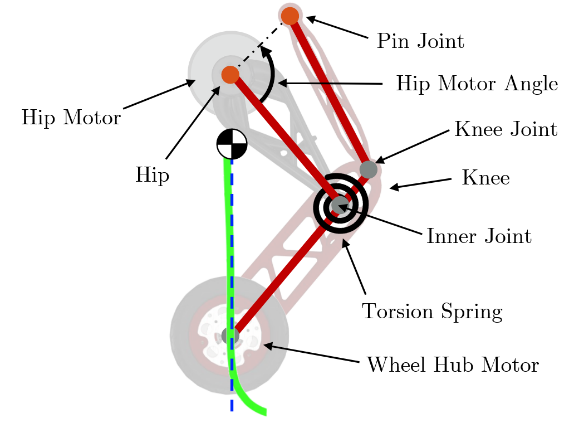
\includegraphics[width=\textwidth]{figures/ch01/image10.png}
  \end{minipage}
  \caption{Ascento 机器人\cite{klemm2019ascento}}
  \label{fig:ascento}
\end{figure}

\begin{figure}[H]
  \centering
  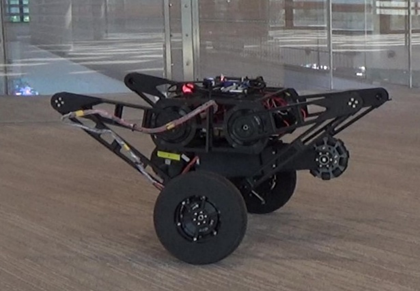
\includegraphics[width=0.52\textwidth]{figures/ch01/image11.png}
  \caption{Ollie 机器人\cite{wang2021ollie}}
  \label{fig:ollie}
\end{figure}

并联构型的共性局限在于：闭链结构天然限制了腿长变化范围和越障高度，且对加工精度与装配误差敏感。Ascento 的有效腿长变化有限，不适合大幅度高度调节；Ollie 依赖额外飞轮补偿空中姿态，增加了控制维度。本文在腿部设计中保留并联支链以获取结构刚度，同时通过将其等效为可伸缩虚拟腿，在任务空间中回避了闭链运动学的复杂性——这在建模思路上与 Ascento 的虚拟腿抽象类似，但在机构形式上以五连杆替代了四连杆。

\subsubsection{混合式结构}

2021 年开源项目 Stanley\cite{stanley2025}（\figref{fig:stanley}）的腿部在运动学上为三自由度串联链，但髋、膝关节的驱动电机并联布置于机身内部，通过绞盘和线缆远程传动，降低了腿部惯量。上海交通大学交龙战队 2025 年开源的双轮足机器人\cite{sjtu2025rm}（\figref{fig:sjtu-hybrid-leg}）同样采用”宏观串联、驱动并联”的混合构型，通过相似连杆机构实现并联传动，并利用导电滑环实现 360° 全向旋转和倒地自起。

\begin{figure}[H]
  \centering
  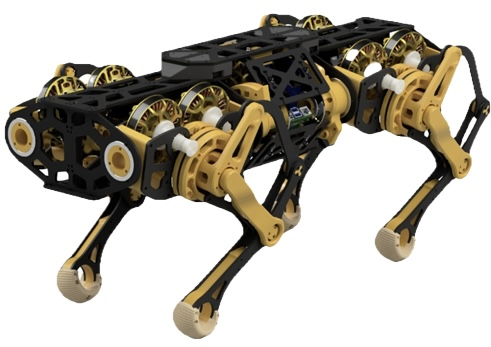
\includegraphics[width=0.38\textwidth]{figures/ch01/image12.jpg}
  \caption{Stanley 机器人\cite{stanley2025}}
  \label{fig:stanley}
\end{figure}

\begin{figure}[H]
  \centering
  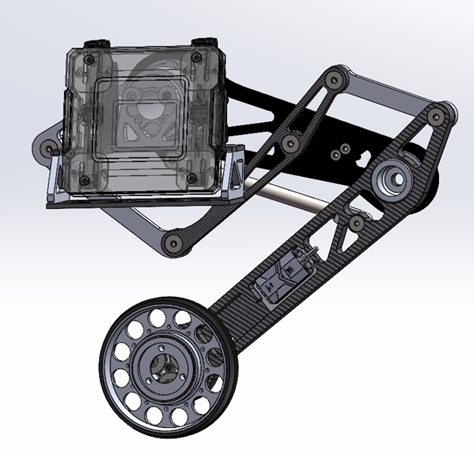
\includegraphics[width=0.4\textwidth]{figures/ch01/image13.png}
  \caption{混合式构型腿部\cite{sjtu2025rm}}
  \label{fig:sjtu-hybrid-leg}
\end{figure}

从上述平台来看，现有混合式方案侧重于将驱动并联化以降低腿部惯量，其闭环支链主要在传动端发挥作用，尚未将并联结构的承载能力直接转化为对轮地接触力和侧向刚度的增强。此外，目前多数平台面向高性能验证或开源竞赛场景，尺寸偏大，缺少面向小型化原型验证的紧凑设计。本文的混合式腿部机构同样遵循”串联主链 + 并联闭环支链”的思路，但将闭环支链直接作用于负载分担和结构刚度提升，而非仅用于传动解耦，这在机构功能定位上与 Stanley 和交龙方案有所区别。

\subsection{运动控制}

双轮足机器人的控制策略融合了轮式平衡与腿式运动两类方法，LQR、VMC、MPC、WBC 和强化学习等均有应用。

Pratt 等人于 2001 年提出虚拟模型控制（VMC）\cite{pratt2001}（\figref{fig:spring-turkey-vmc}），通过模拟虚拟弹簧-阻尼等力学元件直接生成关节力矩，将高层任务描述转化为底层力控指令，显著降低了计算需求。本文的腿长支撑控制直接沿用了这一思想。Sentis 于 2005 年提出全身控制（WBC）框架\cite{sentis2005}，以零空间投影实现多任务的优先级分层，将关节限位、接触约束等硬约束嵌入优化问题，为轮腿系统的多任务协调提供了理论框架。

\begin{figure}[H]
  \centering
  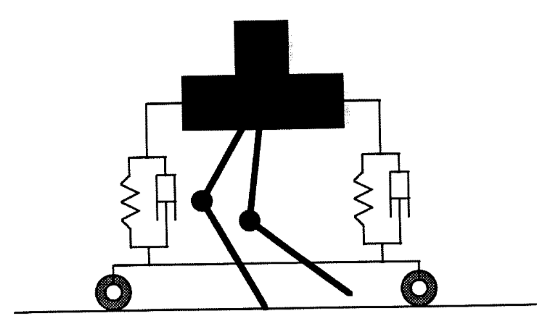
\includegraphics[width=0.6\textwidth]{figures/ch01/image14.png}
  \caption{搭载虚拟助行架的 Spring Turkey 机器人\cite{pratt2001}}
  \label{fig:spring-turkey-vmc}
\end{figure}

在轮式双足机器人的具体应用中，控制方法呈现两条主线。一是以 WBC/MPC 为代表的优化型方法：Klemm 2020 将 LQR 反馈律嵌入 WBC 层级应用于 Ascento\cite{klemm2020lqr}（\figref{fig:lqr-wbc-ascento}），通过闭环力解析解处理腿部运动学闭环，以 ZMP 调节侧倾角抑制侧翻；Wang 2022 提出 MFT-WBC\cite{wang2022mft}（\figref{fig:mft-wbc}），将机构可传递性指标离线建模为多面体约束集成到在线 QP 中，实现了 1\,kHz 伺服速率；Zhang 2022 将自适应动态规划（ADP）与 WBC 结合应用于 Ollie\cite{zhang2022ollie}（\figref{fig:ollie-control-framework}），在线更新控制策略以适应参数变化；Yu 2023 提出轮式刚体动力学（WRBD）模型并结合 MPC 实现 HotWheel 的 6 自由度位姿跟踪\cite{yu2023hotwheel}（\figref{fig:hotwheel-control-framework}）。上述方法的共性是依赖在线优化求解，计算复杂度较高。二是面向特定任务的专项控制：Xia 2025 为双轮足机器人建立了空中动力学模型并设计了跳跃姿态控制器\cite{xia2025jump}（\figref{fig:jump-planning}），验证了基于模型的专项控制在特定动作中的有效性。

\begin{figure}[H]
  \centering
  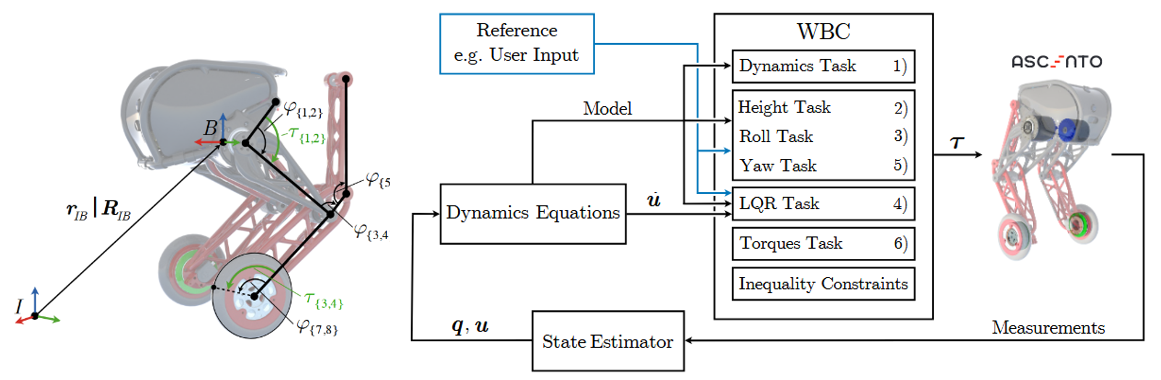
\includegraphics[width=1.0\textwidth]{figures/ch01/image15.png}
  \caption{腿部连杆运动闭环（左），LQR-WBC 控制框架（右）\cite{klemm2020lqr}}
  \label{fig:lqr-wbc-ascento}
\end{figure}

\begin{figure}[H]
  \centering
  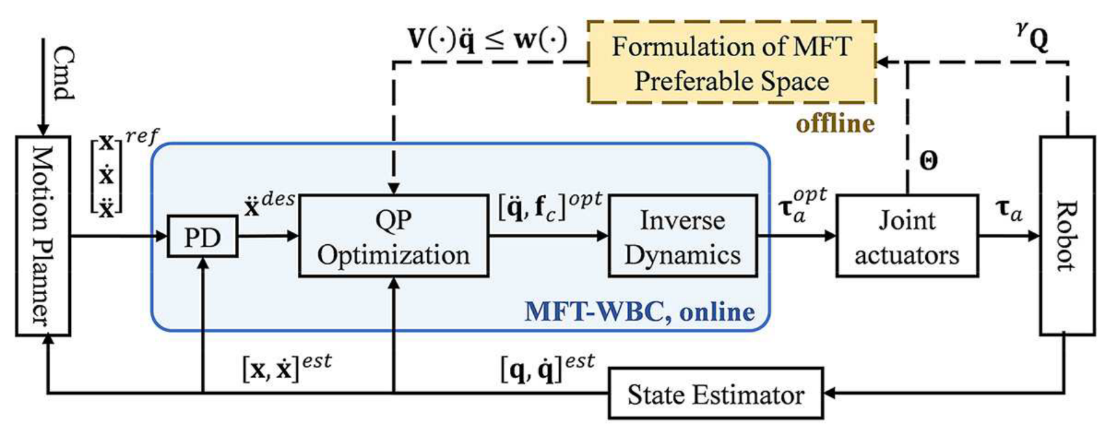
\includegraphics[width=0.72\textwidth]{figures/ch01/image16.png}
  \caption{MFT-WBC 控制框架\cite{wang2022mft}}
  \label{fig:mft-wbc}
\end{figure}

\begin{figure}[H]
  \centering
  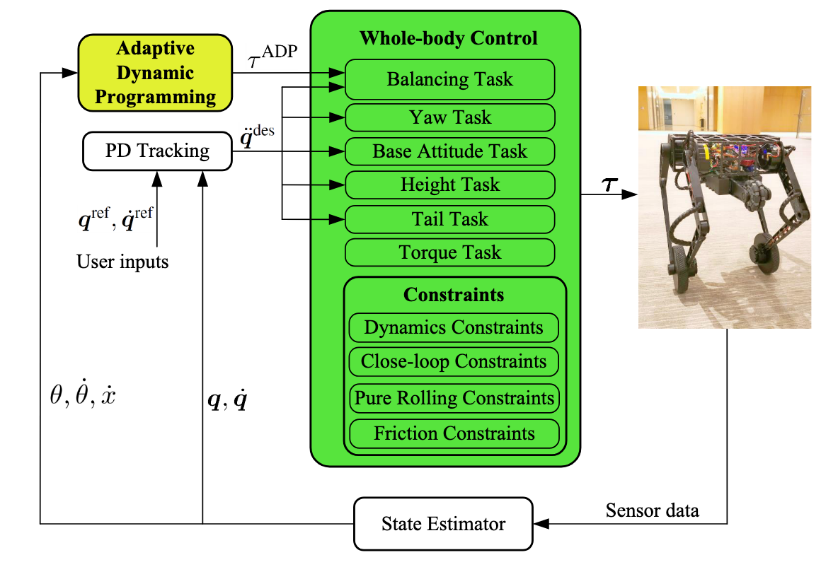
\includegraphics[width=0.65\textwidth]{figures/ch01/image17.png}
  \caption{Ollie 的控制框架\cite{zhang2022ollie}}
  \label{fig:ollie-control-framework}
\end{figure}

\begin{figure}[H]
  \centering
  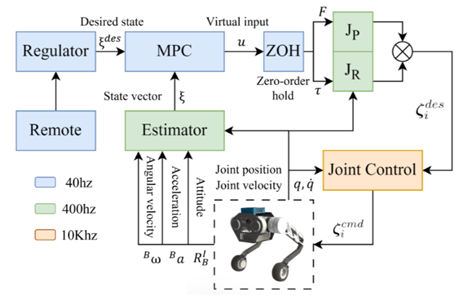
\includegraphics[width=0.7\textwidth]{figures/ch01/image18.png}
  \caption{HotWheel 控制框架\cite{yu2023hotwheel}}
  \label{fig:hotwheel-control-framework}
\end{figure}

\begin{figure}[H]
  \centering
  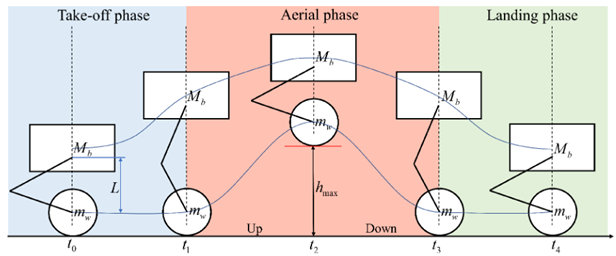
\includegraphics[width=0.8\textwidth]{figures/ch01/image19.png}
  \caption{跳跃过程及轨迹规划示意图\cite{xia2025jump}}
  \label{fig:jump-planning}
\end{figure}

综合来看，优化型方法性能优异但计算成本高，专项控制轻量但覆盖范围有限。本文的分层 LQR-VMC 方案试图在两者之间取折中——以非优化途径实现平衡、腿长支撑和侧向稳定三项核心功能，在不引入在线优化的前提下获得可接受的综合性能。

\begin{table}[H]
  \centering
  \caption{双轮足机器人主流控制方法对比}
  \label{tab:control-method-overview}
  \small
  \begin{tabular}{p{0.9cm}p{2.5cm}p{2.3cm}p{2.5cm}p{3.2cm}}
    \toprule
    方法 & 核心思想 & 优势 & 局限 & 嵌入式实时适用性 \\
    \midrule
    LQR & 平衡点附近线性二次型最优 & 离线求解、在线计算量低 & 需线性化假设，对强非线性适应性有限 & 良好——仅需矩阵乘法 \\
    \hline
    VMC & 虚拟弹簧-阻尼等力学元件直接构造控制量 & 物理直觉强、无需精确模型 & 缺乏多任务协调机制 & 良好——闭式代数运算 \\
    \hline
    WBC & 多任务分层优化，约束优先级处理 & 约束处理完善、多任务协调 & 依赖精确模型 + QP 在线求解 & 较差——每步需解 QP \\
    \hline
    MPC & 滚动时域优化，显式处理约束与预测 & 预测能力强、可处理约束 & 计算量大，对模型精度要求高 & 待提升——TinyMPC 等轻量求解器尚未在轮腿系统验证 \\
    \hline
    RL & 数据驱动、端到端学习控制策略 & 无需显式建模 & 训练数据量大、sim-to-real 差距、可解释性弱 & 部署后可实时推理，但训练阶段成本极高 \\
    \bottomrule
  \end{tabular}
\end{table}

从表\ref{tab:control-method-overview} 可见，WBC 和 MPC 的优越性能以高昂的在线计算为代价，RL 则将复杂性转移到训练阶段。面向嵌入式实时控制的工程需求，LQR 和 VMC 的低计算成本优势突出——前者离线求解 Riccati 方程，在线仅需计算恒定增益矩阵的乘法；后者为闭式代数运算，无需迭代。LQR 和 VMC 的结合能够在保持平衡和腿长支撑两个方向上分别发挥各自优势，且不引入在线优化环节，这正是本文选择 LQR-VMC 分层架构作为控制方案的核心考量。

\subsection{现有研究存在的问题}

现有研究在双轮足机器人的机构设计与控制方法上已取得显著进展，但以下问题仍有待进一步解决。

机械结构方面：串联构型工作空间大，但腿部转动惯量高、刚度不足；并联构型承载能力强、结构紧凑，但运动范围受限、机构复杂。近年来，简化腿部机构以降低驱动与建模复杂度成为一种趋势。Liu 等人在 IROS 2024 提出的 DIABLO 机器人\cite{liu2024diablo} 采用全直驱关节设计，将串联腿部简化为 6 个无减速器电机，并以二阶倒立摆近似其动力学，实现了基于 LQR 的平衡控制。该设计在降低结构复杂度上迈出了重要一步，但其腿部本质上仍为串联构型，未引入并联支链分担关节负载或提升侧向刚度。混合式构型虽试图兼顾两者优势，但现有平台多面向高性能样机验证，在紧凑化、低成本实现方向上的探索尚不充分。

控制方法方面：WBC、MPC 和强化学习等主流策略在复杂任务中控制效果突出，但对高精度模型、在线优化计算或大量训练数据的依赖，使它们在嵌入式平台上面临部署困难、实时性不足等问题。Yu 等人提出的分层 MPC 框架\cite{yu2023mpc} 借助虚拟模型控制思想忽略腿部动力学以降低模型阶数，但 MPC 滚动优化所需的在线求解仍对算力构成较大负担。Nguyen 等人提出的 TinyMPC\cite{nguyen2024tinympc} 获 ICRA 2024 最佳论文奖，通过 ADMM 算法将 MPC 求解压缩至微控制器级别，验证了轻量化优化的可行性，但该方法目前仅在四旋翼上完成验证，尚未拓展至轮腿系统。在 LQR-VMC 混合架构方向上，Yang 等人提出的集成建模与控制优化方案\cite{yang2024integrated} 采用了自适应 LQR 与轨迹方程加速 VMC 相结合的框架，在思路上与本文相近，但其工作以仿真为主，物理实验部分较为初步，缺少完整的闭环验证。对于以工程实现为目标的双轮足机器人，能否在保持平衡、越障和侧向稳定性的同时，降低控制算法的复杂度与实现门槛，仍是一个尚未充分解决的问题。

\section{本文主要研究内容及章节安排}

本文围绕小型混合式双轮足机器人，从机械结构设计、运动学与动力学建模、分层控制方法和实验验证四个方面开展工作。

机械结构方面，完成了整机总体方案与混合式闭环腿部机构设计，以及传动系统、驱动系统的选型与校核，确定了关键结构参数与执行器型号。建模分析方面，建立了机器人的平面等效运动学与动力学模型，推导了面向 LQR 的线性化状态空间表达式，并给出了五连杆机构从任务空间到关节空间的力矩映射关系。控制方法方面，提出了 LQR-VMC 分层控制方案：LQR 负责平衡控制、速度跟踪和腿摆力矩分配，VMC 负责腿长方向的虚拟弹簧-阻尼支撑，同时引入基于滚转角的腿长差修正项以增强侧向姿态的稳定性。在上述工作的基础上，通过仿真和物理样机实验，对原地平衡、速度跟踪、扰动恢复、腿长调节和滚转稳定等典型工况进行了验证。

全文共分为六章，各章节内容安排如下：

第1章为绪论，介绍研究背景与意义，综述双轮足机器人在机械结构与运动控制方面的研究进展，分析现有不足，明确本文的研究内容、技术路线与创新点。

第2章阐述整机总体方案与混合式腿部机构设计，涵盖躯干结构、传动系统、驱动系统及控制硬件的选型与设计，给出关键参数。

第3章建立机器人的平面等效运动学与动力学模型，推导线性化状态空间方程与任务空间到关节空间的力矩映射，为控制器设计提供模型基础。

第4章设计 LQR-VMC 分层控制器，给出状态估计与控制流程，并通过 MuJoCo 仿真验证闭环性能。

第5章在物理样机上开展实验，覆盖原地平衡、速度跟踪、腿长控制和滚转稳定等工况，评估控制器在实际硬件上的性能与稳定性。

第6章总结全文工作与结论，指出当前方法的局限性，展望后续改进方向。

\begin{figure}[H]
  \centering
  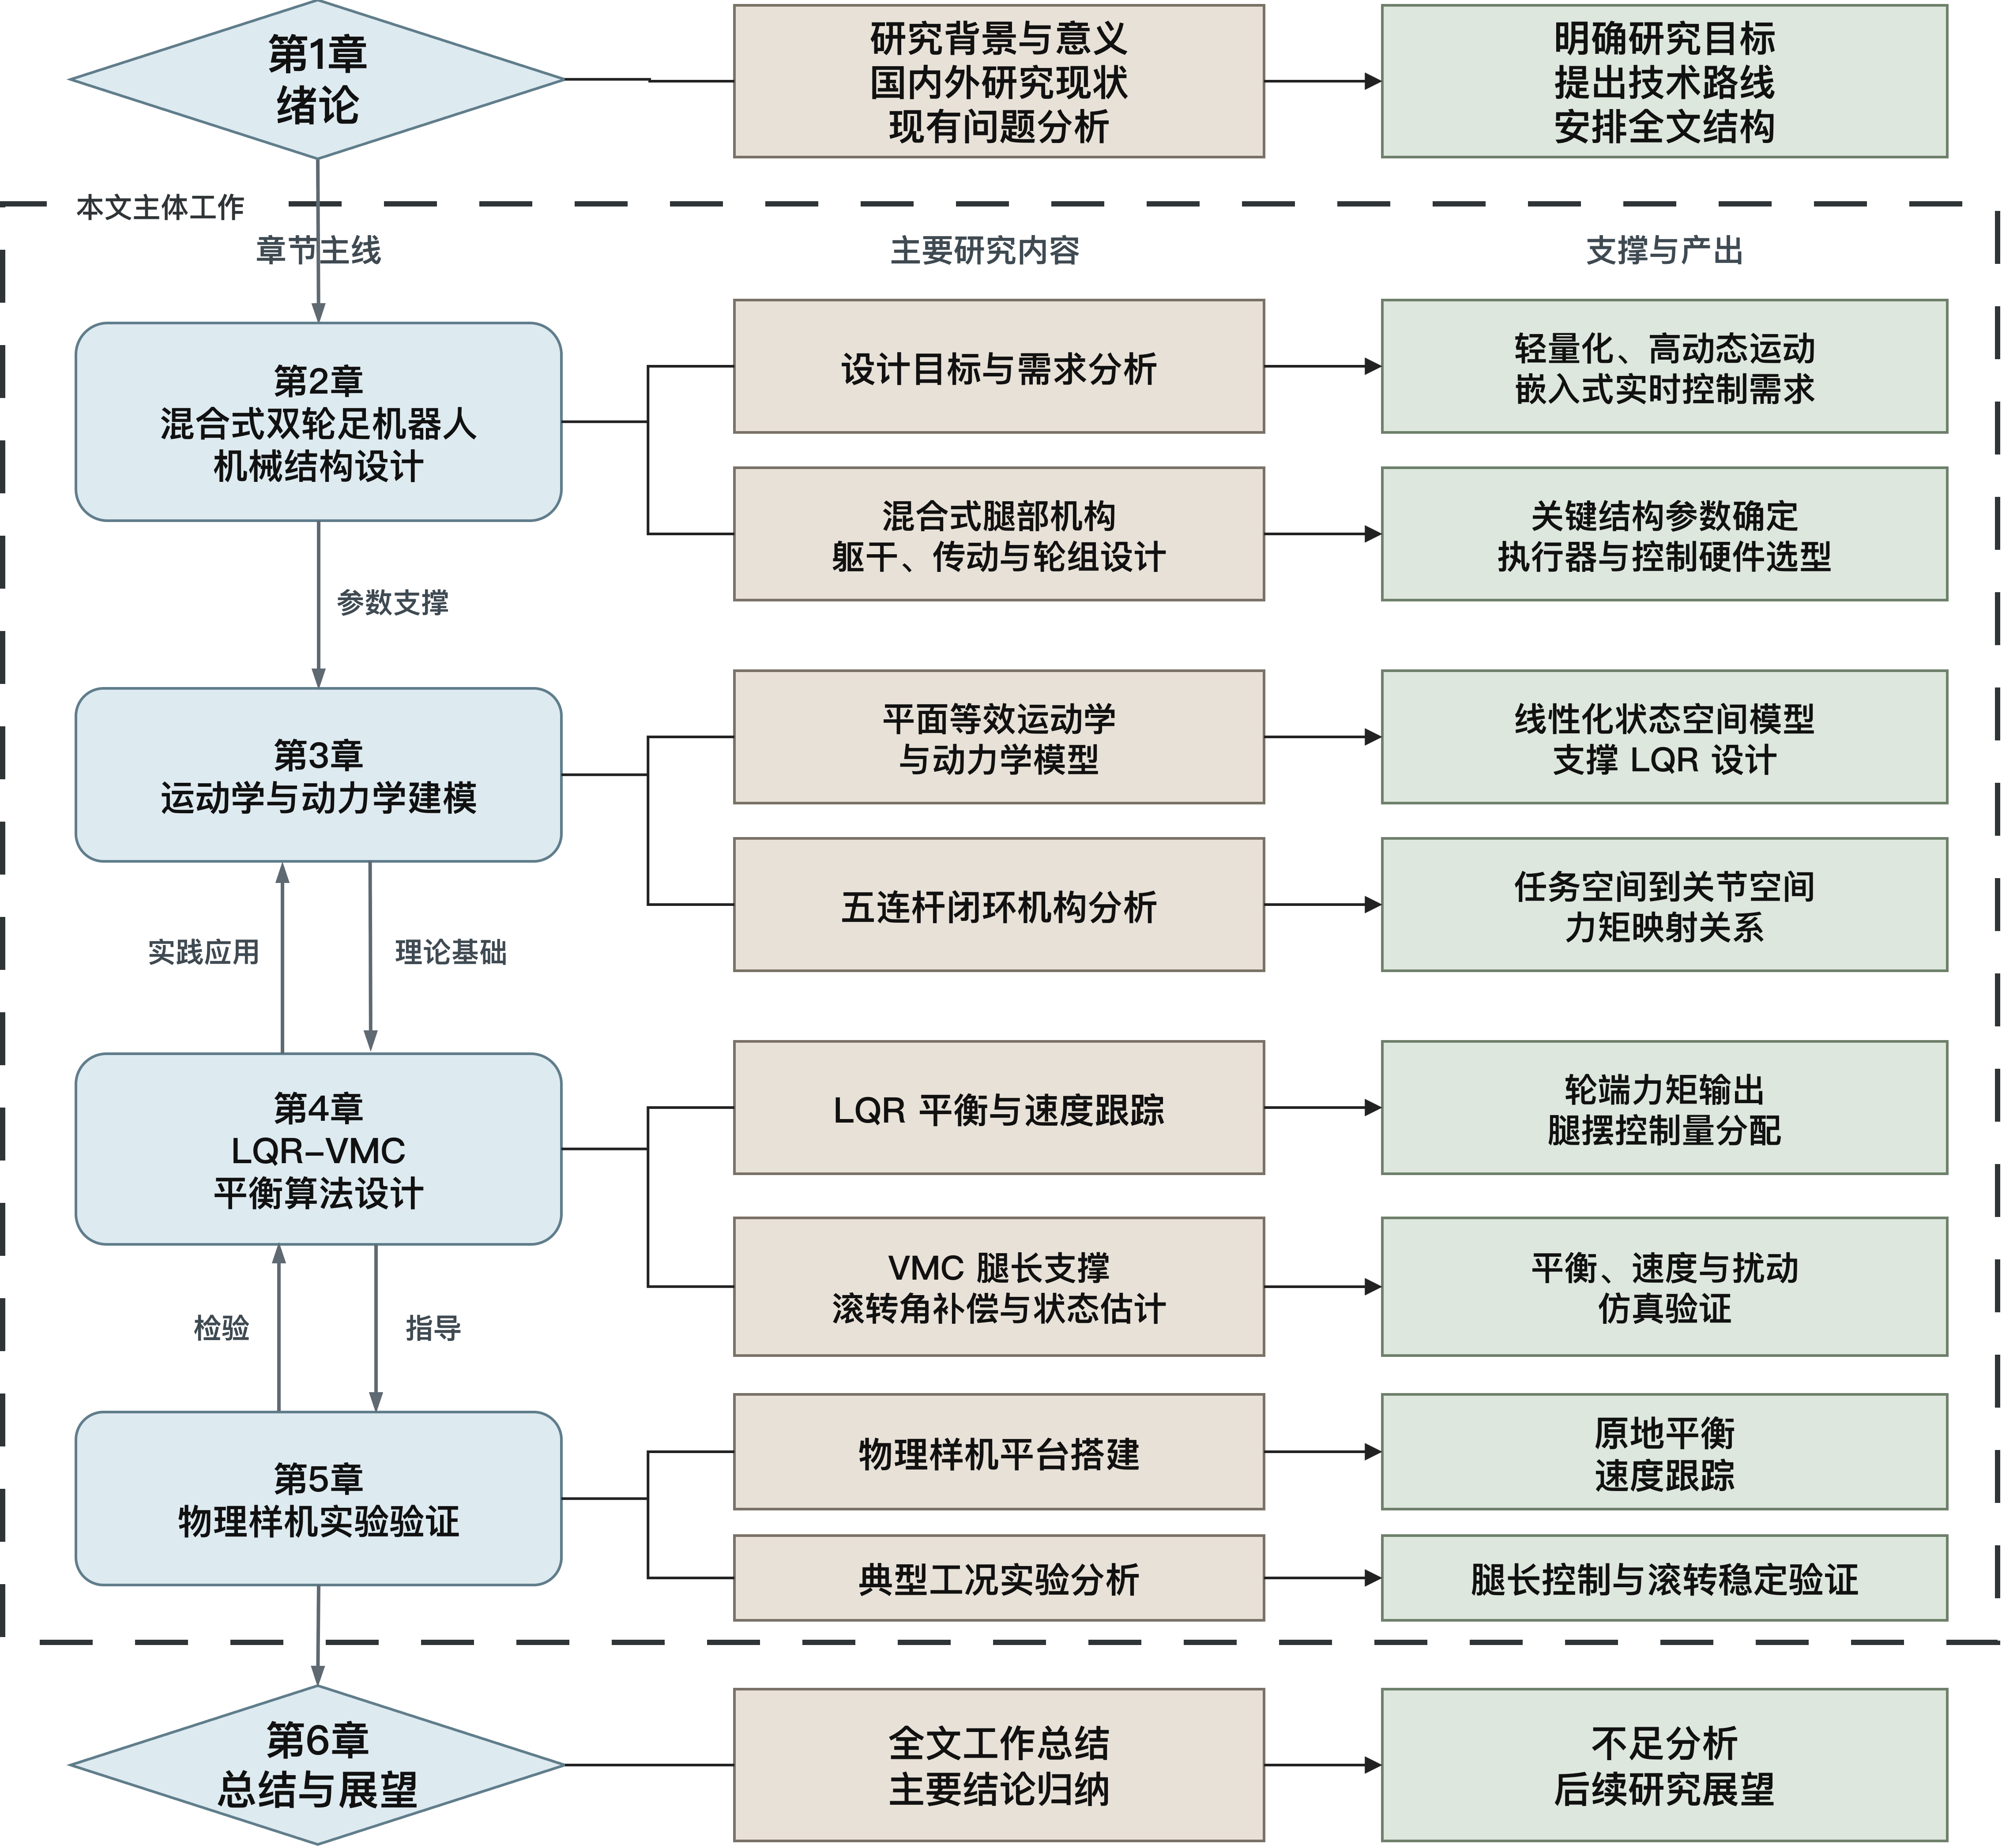
\includegraphics[width=0.9\textwidth]{figures/ch01/research_architecture.png}
  \caption{论文研究内容与技术路线}
  \label{fig:research-architecture}
\end{figure}
